\documentclass[twoside]{book}

% Packages required by doxygen
\usepackage{fixltx2e}
\usepackage{calc}
\usepackage{doxygen}
\usepackage[export]{adjustbox} % also loads graphicx
\usepackage{graphicx}
\usepackage[utf8]{inputenc}
\usepackage{makeidx}
\usepackage{multicol}
\usepackage{multirow}
\PassOptionsToPackage{warn}{textcomp}
\usepackage{textcomp}
\usepackage[nointegrals]{wasysym}
\usepackage[table]{xcolor}

% Font selection
\usepackage[T1]{fontenc}
\usepackage[scaled=.90]{helvet}
\usepackage{courier}
\usepackage{amssymb}
\usepackage{sectsty}
\renewcommand{\familydefault}{\sfdefault}
\allsectionsfont{%
  \fontseries{bc}\selectfont%
  \color{darkgray}%
}
\renewcommand{\DoxyLabelFont}{%
  \fontseries{bc}\selectfont%
  \color{darkgray}%
}
\newcommand{\+}{\discretionary{\mbox{\scriptsize$\hookleftarrow$}}{}{}}

% Page & text layout
\usepackage{geometry}
\geometry{%
  a4paper,%
  top=2.5cm,%
  bottom=2.5cm,%
  left=2.5cm,%
  right=2.5cm%
}
\tolerance=750
\hfuzz=15pt
\hbadness=750
\setlength{\emergencystretch}{15pt}
\setlength{\parindent}{0cm}
\setlength{\parskip}{3ex plus 2ex minus 2ex}
\makeatletter
\renewcommand{\paragraph}{%
  \@startsection{paragraph}{4}{0ex}{-1.0ex}{1.0ex}{%
    \normalfont\normalsize\bfseries\SS@parafont%
  }%
}
\renewcommand{\subparagraph}{%
  \@startsection{subparagraph}{5}{0ex}{-1.0ex}{1.0ex}{%
    \normalfont\normalsize\bfseries\SS@subparafont%
  }%
}
\makeatother

% Headers & footers
\usepackage{fancyhdr}
\pagestyle{fancyplain}
\fancyhead[LE]{\fancyplain{}{\bfseries\thepage}}
\fancyhead[CE]{\fancyplain{}{}}
\fancyhead[RE]{\fancyplain{}{\bfseries\leftmark}}
\fancyhead[LO]{\fancyplain{}{\bfseries\rightmark}}
\fancyhead[CO]{\fancyplain{}{}}
\fancyhead[RO]{\fancyplain{}{\bfseries\thepage}}
\fancyfoot[LE]{\fancyplain{}{}}
\fancyfoot[CE]{\fancyplain{}{}}
\fancyfoot[RE]{\fancyplain{}{\bfseries\scriptsize Generated by Doxygen }}
\fancyfoot[LO]{\fancyplain{}{\bfseries\scriptsize Generated by Doxygen }}
\fancyfoot[CO]{\fancyplain{}{}}
\fancyfoot[RO]{\fancyplain{}{}}
\renewcommand{\footrulewidth}{0.4pt}
\renewcommand{\chaptermark}[1]{%
  \markboth{#1}{}%
}
\renewcommand{\sectionmark}[1]{%
  \markright{\thesection\ #1}%
}

% Indices & bibliography
\usepackage{natbib}
\usepackage[titles]{tocloft}
\setcounter{tocdepth}{3}
\setcounter{secnumdepth}{5}
\makeindex

% Hyperlinks (required, but should be loaded last)
\usepackage{ifpdf}
\ifpdf
  \usepackage[pdftex,pagebackref=true]{hyperref}
\else
  \usepackage[ps2pdf,pagebackref=true]{hyperref}
\fi
\hypersetup{%
  colorlinks=true,%
  linkcolor=blue,%
  citecolor=blue,%
  unicode%
}

% Custom commands
\newcommand{\clearemptydoublepage}{%
  \newpage{\pagestyle{empty}\cleardoublepage}%
}

\usepackage{caption}
\captionsetup{labelsep=space,justification=centering,font={bf},singlelinecheck=off,skip=4pt,position=top}

%===== C O N T E N T S =====

\begin{document}

% Titlepage & ToC
\hypersetup{pageanchor=false,
             bookmarksnumbered=true,
             pdfencoding=unicode
            }
\pagenumbering{alph}
\begin{titlepage}
\vspace*{7cm}
\begin{center}%
{\Large Lotto }\\
\vspace*{1cm}
{\large Generated by Doxygen 1.8.14}\\
\end{center}
\end{titlepage}
\clearemptydoublepage
\pagenumbering{roman}
\tableofcontents
\clearemptydoublepage
\pagenumbering{arabic}
\hypersetup{pageanchor=true}

%--- Begin generated contents ---
\chapter{Namespace Index}
\section{Packages}
Here are the packages with brief descriptions (if available)\+:\begin{DoxyCompactList}
\item\contentsline{section}{\mbox{\hyperlink{namespacemain}{main}} }{\pageref{namespacemain}}{}
\end{DoxyCompactList}

\chapter{Hierarchical Index}
\section{Class Hierarchy}
This inheritance list is sorted roughly, but not completely, alphabetically\+:\begin{DoxyCompactList}
\item \contentsline{section}{Main}{\pageref{classmain_1_1_main}}{}
\item \contentsline{section}{Ruota}{\pageref{classmain_1_1_ruota}}{}
\item \contentsline{section}{Shared\+Data}{\pageref{classmain_1_1_shared_data}}{}
\item Thread\begin{DoxyCompactList}
\item \contentsline{section}{Th\+Cerca}{\pageref{classmain_1_1_th_cerca}}{}
\item \contentsline{section}{Th\+Gen}{\pageref{classmain_1_1_th_gen}}{}
\end{DoxyCompactList}
\end{DoxyCompactList}

\chapter{Class Index}
\section{Class List}
Here are the classes, structs, unions and interfaces with brief descriptions\+:\begin{DoxyCompactList}
\item\contentsline{section}{\mbox{\hyperlink{classmain_1_1_main}{Main}} }{\pageref{classmain_1_1_main}}{}
\item\contentsline{section}{\mbox{\hyperlink{classmain_1_1_ruota}{Ruota}} }{\pageref{classmain_1_1_ruota}}{}
\item\contentsline{section}{\mbox{\hyperlink{classmain_1_1_shared_data}{Shared\+Data}} }{\pageref{classmain_1_1_shared_data}}{}
\item\contentsline{section}{\mbox{\hyperlink{classmain_1_1_th_cerca}{Th\+Cerca}} }{\pageref{classmain_1_1_th_cerca}}{}
\item\contentsline{section}{\mbox{\hyperlink{classmain_1_1_th_gen}{Th\+Gen}} }{\pageref{classmain_1_1_th_gen}}{}
\end{DoxyCompactList}

\chapter{File Index}
\section{File List}
Here is a list of all files with brief descriptions\+:\begin{DoxyCompactList}
\item\contentsline{section}{C\+:/\+Users/\+Luca Mantica/\+Desktop/\+Scuola/4 anno/\+Tecnologie/\+Java/\+Repositories/\+Lotto/\+Lotto/src/main/\mbox{\hyperlink{_main_8java}{Main.\+java}} }{\pageref{_main_8java}}{}
\item\contentsline{section}{C\+:/\+Users/\+Luca Mantica/\+Desktop/\+Scuola/4 anno/\+Tecnologie/\+Java/\+Repositories/\+Lotto/\+Lotto/src/main/\mbox{\hyperlink{_ruota_8java}{Ruota.\+java}} }{\pageref{_ruota_8java}}{}
\item\contentsline{section}{C\+:/\+Users/\+Luca Mantica/\+Desktop/\+Scuola/4 anno/\+Tecnologie/\+Java/\+Repositories/\+Lotto/\+Lotto/src/main/\mbox{\hyperlink{_shared_data_8java}{Shared\+Data.\+java}} }{\pageref{_shared_data_8java}}{}
\item\contentsline{section}{C\+:/\+Users/\+Luca Mantica/\+Desktop/\+Scuola/4 anno/\+Tecnologie/\+Java/\+Repositories/\+Lotto/\+Lotto/src/main/\mbox{\hyperlink{_th_cerca_8java}{Th\+Cerca.\+java}} }{\pageref{_th_cerca_8java}}{}
\item\contentsline{section}{C\+:/\+Users/\+Luca Mantica/\+Desktop/\+Scuola/4 anno/\+Tecnologie/\+Java/\+Repositories/\+Lotto/\+Lotto/src/main/\mbox{\hyperlink{_th_gen_8java}{Th\+Gen.\+java}} }{\pageref{_th_gen_8java}}{}
\end{DoxyCompactList}

\chapter{Namespace Documentation}
\hypertarget{namespacemain}{}\section{Package main}
\label{namespacemain}\index{main@{main}}
\subsection*{Classes}
\begin{DoxyCompactItemize}
\item 
class \mbox{\hyperlink{classmain_1_1_main}{Main}}
\item 
class \mbox{\hyperlink{classmain_1_1_ruota}{Ruota}}
\item 
class \mbox{\hyperlink{classmain_1_1_shared_data}{Shared\+Data}}
\item 
class \mbox{\hyperlink{classmain_1_1_th_cerca}{Th\+Cerca}}
\item 
class \mbox{\hyperlink{classmain_1_1_th_gen}{Th\+Gen}}
\end{DoxyCompactItemize}

\chapter{Class Documentation}
\hypertarget{classmain_1_1_main}{}\section{Main Class Reference}
\label{classmain_1_1_main}\index{Main@{Main}}


Collaboration diagram for Main\+:
\nopagebreak
\begin{figure}[H]
\begin{center}
\leavevmode
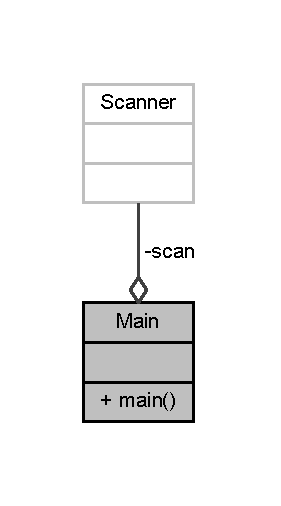
\includegraphics[width=135pt]{classmain_1_1_main__coll__graph}
\end{center}
\end{figure}
\subsection*{Static Public Member Functions}
\begin{DoxyCompactItemize}
\item 
static void \mbox{\hyperlink{classmain_1_1_main_a8b260eecbaabcef8473fd87ada040682}{main}} (String\mbox{[}$\,$\mbox{]} args)
\end{DoxyCompactItemize}
\subsection*{Static Private Attributes}
\begin{DoxyCompactItemize}
\item 
static final Scanner \mbox{\hyperlink{classmain_1_1_main_ad2b26d92ead66c3a1c4e4d4d77394aba}{scan}} = new Scanner(System.\+in)
\end{DoxyCompactItemize}


\subsection{Detailed Description}


Definition at line 8 of file Main.\+java.



\subsection{Member Function Documentation}
\mbox{\Hypertarget{classmain_1_1_main_a8b260eecbaabcef8473fd87ada040682}\label{classmain_1_1_main_a8b260eecbaabcef8473fd87ada040682}} 
\index{main\+::\+Main@{main\+::\+Main}!main@{main}}
\index{main@{main}!main\+::\+Main@{main\+::\+Main}}
\subsubsection{\texorpdfstring{main()}{main()}}
{\footnotesize\ttfamily static void main (\begin{DoxyParamCaption}\item[{String \mbox{[}$\,$\mbox{]}}]{args }\end{DoxyParamCaption})\hspace{0.3cm}{\ttfamily [static]}}



Definition at line 12 of file Main.\+java.

Here is the call graph for this function\+:
\nopagebreak
\begin{figure}[H]
\begin{center}
\leavevmode
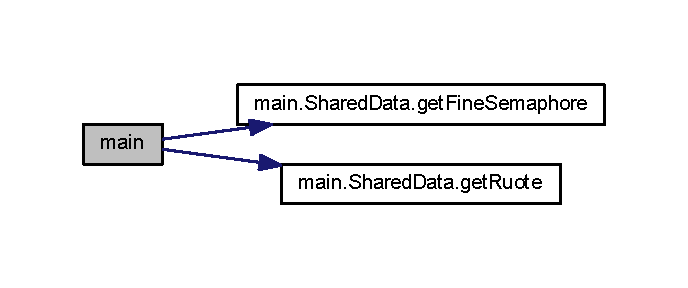
\includegraphics[width=330pt]{classmain_1_1_main_a8b260eecbaabcef8473fd87ada040682_cgraph}
\end{center}
\end{figure}


\subsection{Member Data Documentation}
\mbox{\Hypertarget{classmain_1_1_main_ad2b26d92ead66c3a1c4e4d4d77394aba}\label{classmain_1_1_main_ad2b26d92ead66c3a1c4e4d4d77394aba}} 
\index{main\+::\+Main@{main\+::\+Main}!scan@{scan}}
\index{scan@{scan}!main\+::\+Main@{main\+::\+Main}}
\subsubsection{\texorpdfstring{scan}{scan}}
{\footnotesize\ttfamily final Scanner scan = new Scanner(System.\+in)\hspace{0.3cm}{\ttfamily [static]}, {\ttfamily [private]}}



Definition at line 10 of file Main.\+java.



The documentation for this class was generated from the following file\+:\begin{DoxyCompactItemize}
\item 
C\+:/\+Users/\+Luca Mantica/\+Desktop/\+Scuola/4 anno/\+Tecnologie/\+Java/\+Repositories/\+Lotto/\+Lotto/src/main/\mbox{\hyperlink{_main_8java}{Main.\+java}}\end{DoxyCompactItemize}

\hypertarget{classmain_1_1_ruota}{}\section{Ruota Class Reference}
\label{classmain_1_1_ruota}\index{Ruota@{Ruota}}


Collaboration diagram for Ruota\+:
\nopagebreak
\begin{figure}[H]
\begin{center}
\leavevmode
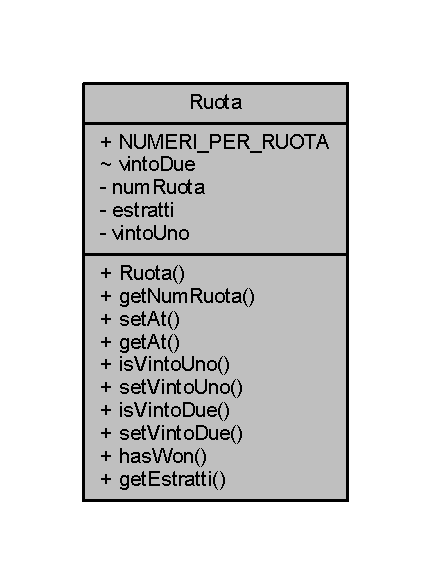
\includegraphics[width=207pt]{classmain_1_1_ruota__coll__graph}
\end{center}
\end{figure}
\subsection*{Public Member Functions}
\begin{DoxyCompactItemize}
\item 
\mbox{\hyperlink{classmain_1_1_ruota_a94f55777c902bce8766a98bb0423b7a0}{Ruota}} (int \mbox{\hyperlink{classmain_1_1_ruota_ab7691d77fe75980e207c3c89cf90b7da}{num\+Ruota}})
\item 
synchronized int \mbox{\hyperlink{classmain_1_1_ruota_a42fe6d0ed82bf794b0956983a6b5f8b2}{get\+Num\+Ruota}} ()
\item 
synchronized void \mbox{\hyperlink{classmain_1_1_ruota_a3debdaf5d71e61062f8c3ac4bfba02b8}{set\+At}} (int index, int val)
\item 
synchronized int \mbox{\hyperlink{classmain_1_1_ruota_a3fbe06494cd4fa2d6fd022c2e84e9156}{get\+At}} (int index)
\item 
synchronized boolean \mbox{\hyperlink{classmain_1_1_ruota_ae2a86522fbeb35b9286bf2a14f663186}{is\+Vinto\+Uno}} ()
\item 
synchronized void \mbox{\hyperlink{classmain_1_1_ruota_a24f43a149e8280c81c9718eada8ece10}{set\+Vinto\+Uno}} (boolean \mbox{\hyperlink{classmain_1_1_ruota_a208227a3e29bd1d579feb423a9948700}{vinto\+Uno}})
\item 
synchronized boolean \mbox{\hyperlink{classmain_1_1_ruota_afd35315bdd4e0c12efd6d410f9573784}{is\+Vinto\+Due}} ()
\item 
synchronized void \mbox{\hyperlink{classmain_1_1_ruota_ab033e20bad03089115af5905cd091752}{set\+Vinto\+Due}} (boolean vinto\+Due)
\item 
synchronized boolean \mbox{\hyperlink{classmain_1_1_ruota_aed75271bb2c21c3cb7e838a2cdc1898a}{has\+Won}} ()
\item 
int \mbox{[}$\,$\mbox{]} \mbox{\hyperlink{classmain_1_1_ruota_a0dee4d8069c9f083fac5bd060b9ae872}{get\+Estratti}} ()
\end{DoxyCompactItemize}
\subsection*{Static Public Attributes}
\begin{DoxyCompactItemize}
\item 
static final int \mbox{\hyperlink{classmain_1_1_ruota_a545c7333f82d918fed8d2a5838c334fd}{N\+U\+M\+E\+R\+I\+\_\+\+P\+E\+R\+\_\+\+R\+U\+O\+TA}} = 5
\end{DoxyCompactItemize}
\subsection*{Private Attributes}
\begin{DoxyCompactItemize}
\item 
final int \mbox{\hyperlink{classmain_1_1_ruota_ab7691d77fe75980e207c3c89cf90b7da}{num\+Ruota}}
\item 
int \mbox{[}$\,$\mbox{]} \mbox{\hyperlink{classmain_1_1_ruota_a7be91eda031da75cc73826a2a0196c6c}{estratti}}
\item 
boolean \mbox{\hyperlink{classmain_1_1_ruota_a208227a3e29bd1d579feb423a9948700}{vinto\+Uno}}
\end{DoxyCompactItemize}


\subsection{Detailed Description}


Definition at line 3 of file Ruota.\+java.



\subsection{Constructor \& Destructor Documentation}
\mbox{\Hypertarget{classmain_1_1_ruota_a94f55777c902bce8766a98bb0423b7a0}\label{classmain_1_1_ruota_a94f55777c902bce8766a98bb0423b7a0}} 
\index{main\+::\+Ruota@{main\+::\+Ruota}!Ruota@{Ruota}}
\index{Ruota@{Ruota}!main\+::\+Ruota@{main\+::\+Ruota}}
\subsubsection{\texorpdfstring{Ruota()}{Ruota()}}
{\footnotesize\ttfamily \mbox{\hyperlink{classmain_1_1_ruota}{Ruota}} (\begin{DoxyParamCaption}\item[{int}]{num\+Ruota }\end{DoxyParamCaption})}



Definition at line 10 of file Ruota.\+java.



\subsection{Member Function Documentation}
\mbox{\Hypertarget{classmain_1_1_ruota_a3fbe06494cd4fa2d6fd022c2e84e9156}\label{classmain_1_1_ruota_a3fbe06494cd4fa2d6fd022c2e84e9156}} 
\index{main\+::\+Ruota@{main\+::\+Ruota}!get\+At@{get\+At}}
\index{get\+At@{get\+At}!main\+::\+Ruota@{main\+::\+Ruota}}
\subsubsection{\texorpdfstring{get\+At()}{getAt()}}
{\footnotesize\ttfamily synchronized int get\+At (\begin{DoxyParamCaption}\item[{int}]{index }\end{DoxyParamCaption})}



Definition at line 25 of file Ruota.\+java.

\mbox{\Hypertarget{classmain_1_1_ruota_a0dee4d8069c9f083fac5bd060b9ae872}\label{classmain_1_1_ruota_a0dee4d8069c9f083fac5bd060b9ae872}} 
\index{main\+::\+Ruota@{main\+::\+Ruota}!get\+Estratti@{get\+Estratti}}
\index{get\+Estratti@{get\+Estratti}!main\+::\+Ruota@{main\+::\+Ruota}}
\subsubsection{\texorpdfstring{get\+Estratti()}{getEstratti()}}
{\footnotesize\ttfamily int \mbox{[}$\,$\mbox{]} get\+Estratti (\begin{DoxyParamCaption}{ }\end{DoxyParamCaption})}



Definition at line 49 of file Ruota.\+java.

\mbox{\Hypertarget{classmain_1_1_ruota_a42fe6d0ed82bf794b0956983a6b5f8b2}\label{classmain_1_1_ruota_a42fe6d0ed82bf794b0956983a6b5f8b2}} 
\index{main\+::\+Ruota@{main\+::\+Ruota}!get\+Num\+Ruota@{get\+Num\+Ruota}}
\index{get\+Num\+Ruota@{get\+Num\+Ruota}!main\+::\+Ruota@{main\+::\+Ruota}}
\subsubsection{\texorpdfstring{get\+Num\+Ruota()}{getNumRuota()}}
{\footnotesize\ttfamily synchronized int get\+Num\+Ruota (\begin{DoxyParamCaption}{ }\end{DoxyParamCaption})}



Definition at line 17 of file Ruota.\+java.

\mbox{\Hypertarget{classmain_1_1_ruota_aed75271bb2c21c3cb7e838a2cdc1898a}\label{classmain_1_1_ruota_aed75271bb2c21c3cb7e838a2cdc1898a}} 
\index{main\+::\+Ruota@{main\+::\+Ruota}!has\+Won@{has\+Won}}
\index{has\+Won@{has\+Won}!main\+::\+Ruota@{main\+::\+Ruota}}
\subsubsection{\texorpdfstring{has\+Won()}{hasWon()}}
{\footnotesize\ttfamily synchronized boolean has\+Won (\begin{DoxyParamCaption}{ }\end{DoxyParamCaption})}



Definition at line 45 of file Ruota.\+java.

\mbox{\Hypertarget{classmain_1_1_ruota_afd35315bdd4e0c12efd6d410f9573784}\label{classmain_1_1_ruota_afd35315bdd4e0c12efd6d410f9573784}} 
\index{main\+::\+Ruota@{main\+::\+Ruota}!is\+Vinto\+Due@{is\+Vinto\+Due}}
\index{is\+Vinto\+Due@{is\+Vinto\+Due}!main\+::\+Ruota@{main\+::\+Ruota}}
\subsubsection{\texorpdfstring{is\+Vinto\+Due()}{isVintoDue()}}
{\footnotesize\ttfamily synchronized boolean is\+Vinto\+Due (\begin{DoxyParamCaption}{ }\end{DoxyParamCaption})}



Definition at line 37 of file Ruota.\+java.

\mbox{\Hypertarget{classmain_1_1_ruota_ae2a86522fbeb35b9286bf2a14f663186}\label{classmain_1_1_ruota_ae2a86522fbeb35b9286bf2a14f663186}} 
\index{main\+::\+Ruota@{main\+::\+Ruota}!is\+Vinto\+Uno@{is\+Vinto\+Uno}}
\index{is\+Vinto\+Uno@{is\+Vinto\+Uno}!main\+::\+Ruota@{main\+::\+Ruota}}
\subsubsection{\texorpdfstring{is\+Vinto\+Uno()}{isVintoUno()}}
{\footnotesize\ttfamily synchronized boolean is\+Vinto\+Uno (\begin{DoxyParamCaption}{ }\end{DoxyParamCaption})}



Definition at line 29 of file Ruota.\+java.

\mbox{\Hypertarget{classmain_1_1_ruota_a3debdaf5d71e61062f8c3ac4bfba02b8}\label{classmain_1_1_ruota_a3debdaf5d71e61062f8c3ac4bfba02b8}} 
\index{main\+::\+Ruota@{main\+::\+Ruota}!set\+At@{set\+At}}
\index{set\+At@{set\+At}!main\+::\+Ruota@{main\+::\+Ruota}}
\subsubsection{\texorpdfstring{set\+At()}{setAt()}}
{\footnotesize\ttfamily synchronized void set\+At (\begin{DoxyParamCaption}\item[{int}]{index,  }\item[{int}]{val }\end{DoxyParamCaption})}



Definition at line 21 of file Ruota.\+java.

\mbox{\Hypertarget{classmain_1_1_ruota_ab033e20bad03089115af5905cd091752}\label{classmain_1_1_ruota_ab033e20bad03089115af5905cd091752}} 
\index{main\+::\+Ruota@{main\+::\+Ruota}!set\+Vinto\+Due@{set\+Vinto\+Due}}
\index{set\+Vinto\+Due@{set\+Vinto\+Due}!main\+::\+Ruota@{main\+::\+Ruota}}
\subsubsection{\texorpdfstring{set\+Vinto\+Due()}{setVintoDue()}}
{\footnotesize\ttfamily synchronized void set\+Vinto\+Due (\begin{DoxyParamCaption}\item[{boolean}]{vinto\+Due }\end{DoxyParamCaption})}



Definition at line 41 of file Ruota.\+java.

\mbox{\Hypertarget{classmain_1_1_ruota_a24f43a149e8280c81c9718eada8ece10}\label{classmain_1_1_ruota_a24f43a149e8280c81c9718eada8ece10}} 
\index{main\+::\+Ruota@{main\+::\+Ruota}!set\+Vinto\+Uno@{set\+Vinto\+Uno}}
\index{set\+Vinto\+Uno@{set\+Vinto\+Uno}!main\+::\+Ruota@{main\+::\+Ruota}}
\subsubsection{\texorpdfstring{set\+Vinto\+Uno()}{setVintoUno()}}
{\footnotesize\ttfamily synchronized void set\+Vinto\+Uno (\begin{DoxyParamCaption}\item[{boolean}]{vinto\+Uno }\end{DoxyParamCaption})}



Definition at line 33 of file Ruota.\+java.



\subsection{Member Data Documentation}
\mbox{\Hypertarget{classmain_1_1_ruota_a7be91eda031da75cc73826a2a0196c6c}\label{classmain_1_1_ruota_a7be91eda031da75cc73826a2a0196c6c}} 
\index{main\+::\+Ruota@{main\+::\+Ruota}!estratti@{estratti}}
\index{estratti@{estratti}!main\+::\+Ruota@{main\+::\+Ruota}}
\subsubsection{\texorpdfstring{estratti}{estratti}}
{\footnotesize\ttfamily int \mbox{[}$\,$\mbox{]} estratti\hspace{0.3cm}{\ttfamily [private]}}



Definition at line 7 of file Ruota.\+java.

\mbox{\Hypertarget{classmain_1_1_ruota_a545c7333f82d918fed8d2a5838c334fd}\label{classmain_1_1_ruota_a545c7333f82d918fed8d2a5838c334fd}} 
\index{main\+::\+Ruota@{main\+::\+Ruota}!N\+U\+M\+E\+R\+I\+\_\+\+P\+E\+R\+\_\+\+R\+U\+O\+TA@{N\+U\+M\+E\+R\+I\+\_\+\+P\+E\+R\+\_\+\+R\+U\+O\+TA}}
\index{N\+U\+M\+E\+R\+I\+\_\+\+P\+E\+R\+\_\+\+R\+U\+O\+TA@{N\+U\+M\+E\+R\+I\+\_\+\+P\+E\+R\+\_\+\+R\+U\+O\+TA}!main\+::\+Ruota@{main\+::\+Ruota}}
\subsubsection{\texorpdfstring{N\+U\+M\+E\+R\+I\+\_\+\+P\+E\+R\+\_\+\+R\+U\+O\+TA}{NUMERI\_PER\_RUOTA}}
{\footnotesize\ttfamily final int N\+U\+M\+E\+R\+I\+\_\+\+P\+E\+R\+\_\+\+R\+U\+O\+TA = 5\hspace{0.3cm}{\ttfamily [static]}}



Definition at line 4 of file Ruota.\+java.

\mbox{\Hypertarget{classmain_1_1_ruota_ab7691d77fe75980e207c3c89cf90b7da}\label{classmain_1_1_ruota_ab7691d77fe75980e207c3c89cf90b7da}} 
\index{main\+::\+Ruota@{main\+::\+Ruota}!num\+Ruota@{num\+Ruota}}
\index{num\+Ruota@{num\+Ruota}!main\+::\+Ruota@{main\+::\+Ruota}}
\subsubsection{\texorpdfstring{num\+Ruota}{numRuota}}
{\footnotesize\ttfamily final int num\+Ruota\hspace{0.3cm}{\ttfamily [private]}}



Definition at line 6 of file Ruota.\+java.

\mbox{\Hypertarget{classmain_1_1_ruota_a208227a3e29bd1d579feb423a9948700}\label{classmain_1_1_ruota_a208227a3e29bd1d579feb423a9948700}} 
\index{main\+::\+Ruota@{main\+::\+Ruota}!vinto\+Uno@{vinto\+Uno}}
\index{vinto\+Uno@{vinto\+Uno}!main\+::\+Ruota@{main\+::\+Ruota}}
\subsubsection{\texorpdfstring{vinto\+Uno}{vintoUno}}
{\footnotesize\ttfamily boolean vinto\+Uno\hspace{0.3cm}{\ttfamily [private]}}



Definition at line 8 of file Ruota.\+java.



The documentation for this class was generated from the following file\+:\begin{DoxyCompactItemize}
\item 
C\+:/\+Users/\+Luca Mantica/\+Desktop/\+Scuola/4 anno/\+Tecnologie/\+Java/\+Repositories/\+Lotto/\+Lotto/src/main/\mbox{\hyperlink{_ruota_8java}{Ruota.\+java}}\end{DoxyCompactItemize}

\hypertarget{classmain_1_1_shared_data}{}\section{Shared\+Data Class Reference}
\label{classmain_1_1_shared_data}\index{Shared\+Data@{Shared\+Data}}


Collaboration diagram for Shared\+Data\+:
\nopagebreak
\begin{figure}[H]
\begin{center}
\leavevmode
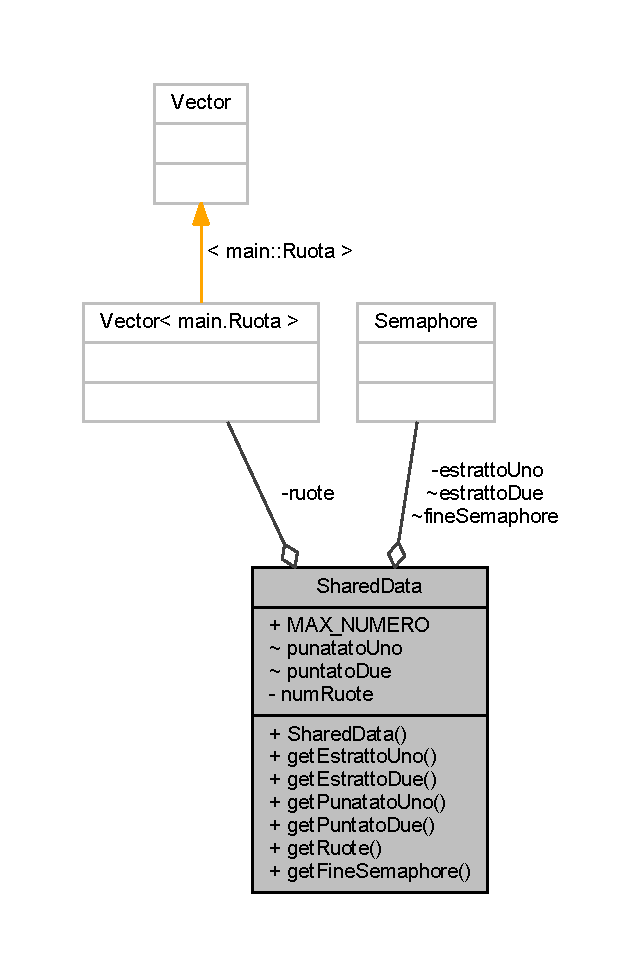
\includegraphics[width=309pt]{classmain_1_1_shared_data__coll__graph}
\end{center}
\end{figure}
\subsection*{Public Member Functions}
\begin{DoxyCompactItemize}
\item 
\mbox{\hyperlink{classmain_1_1_shared_data_a7c3fcf7e88661c8f19dc4f1bef3b1f1c}{Shared\+Data}} (int \mbox{\hyperlink{classmain_1_1_shared_data_afd761d5f372b32a47d35514239540df6}{num\+Ruote}}, int punatato\+Uno, int puntato\+Due)
\item 
synchronized Semaphore \mbox{\hyperlink{classmain_1_1_shared_data_a113b8bd4e0520f7610c30c826d177898}{get\+Estratto\+Uno}} ()
\item 
synchronized Semaphore \mbox{\hyperlink{classmain_1_1_shared_data_a03babbf5685e678be2baebb70af3fc4e}{get\+Estratto\+Due}} ()
\item 
synchronized int \mbox{\hyperlink{classmain_1_1_shared_data_a61e4168cef037c5305a703af0c3e5ce5}{get\+Punatato\+Uno}} ()
\item 
synchronized int \mbox{\hyperlink{classmain_1_1_shared_data_afe476c2ad5a76e2d77871f0cfe94b1fd}{get\+Puntato\+Due}} ()
\item 
synchronized Vector$<$ \mbox{\hyperlink{classmain_1_1_ruota}{Ruota}} $>$ \mbox{\hyperlink{classmain_1_1_shared_data_aa492c5b4f3fb55eb33f9c79b7b484d41}{get\+Ruote}} ()
\item 
synchronized Semaphore \mbox{\hyperlink{classmain_1_1_shared_data_ab9a75de14be42bfeb3654d44f09b20bf}{get\+Fine\+Semaphore}} ()
\end{DoxyCompactItemize}
\subsection*{Static Public Attributes}
\begin{DoxyCompactItemize}
\item 
static final int \mbox{\hyperlink{classmain_1_1_shared_data_af9e82eed5f04a857c2749dae6956ddc1}{M\+A\+X\+\_\+\+N\+U\+M\+E\+RO}} = 99
\end{DoxyCompactItemize}
\subsection*{Private Attributes}
\begin{DoxyCompactItemize}
\item 
Vector$<$ \mbox{\hyperlink{classmain_1_1_ruota}{Ruota}} $>$ \mbox{\hyperlink{classmain_1_1_shared_data_a3336af22f48845590e6b9cace9d82ce1}{ruote}}
\item 
final int \mbox{\hyperlink{classmain_1_1_shared_data_afd761d5f372b32a47d35514239540df6}{num\+Ruote}}
\item 
final Semaphore \mbox{\hyperlink{classmain_1_1_shared_data_a63712f23e96673948c3fd3c48b64d05b}{estratto\+Uno}}
\end{DoxyCompactItemize}


\subsection{Detailed Description}


Definition at line 6 of file Shared\+Data.\+java.



\subsection{Constructor \& Destructor Documentation}
\mbox{\Hypertarget{classmain_1_1_shared_data_a7c3fcf7e88661c8f19dc4f1bef3b1f1c}\label{classmain_1_1_shared_data_a7c3fcf7e88661c8f19dc4f1bef3b1f1c}} 
\index{main\+::\+Shared\+Data@{main\+::\+Shared\+Data}!Shared\+Data@{Shared\+Data}}
\index{Shared\+Data@{Shared\+Data}!main\+::\+Shared\+Data@{main\+::\+Shared\+Data}}
\subsubsection{\texorpdfstring{Shared\+Data()}{SharedData()}}
{\footnotesize\ttfamily \mbox{\hyperlink{classmain_1_1_shared_data}{Shared\+Data}} (\begin{DoxyParamCaption}\item[{int}]{num\+Ruote,  }\item[{int}]{punatato\+Uno,  }\item[{int}]{puntato\+Due }\end{DoxyParamCaption})}



Definition at line 13 of file Shared\+Data.\+java.



\subsection{Member Function Documentation}
\mbox{\Hypertarget{classmain_1_1_shared_data_a03babbf5685e678be2baebb70af3fc4e}\label{classmain_1_1_shared_data_a03babbf5685e678be2baebb70af3fc4e}} 
\index{main\+::\+Shared\+Data@{main\+::\+Shared\+Data}!get\+Estratto\+Due@{get\+Estratto\+Due}}
\index{get\+Estratto\+Due@{get\+Estratto\+Due}!main\+::\+Shared\+Data@{main\+::\+Shared\+Data}}
\subsubsection{\texorpdfstring{get\+Estratto\+Due()}{getEstrattoDue()}}
{\footnotesize\ttfamily synchronized Semaphore get\+Estratto\+Due (\begin{DoxyParamCaption}{ }\end{DoxyParamCaption})}



Definition at line 30 of file Shared\+Data.\+java.

Here is the caller graph for this function\+:
\nopagebreak
\begin{figure}[H]
\begin{center}
\leavevmode
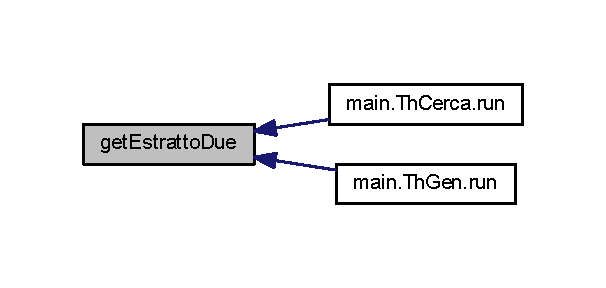
\includegraphics[width=291pt]{classmain_1_1_shared_data_a03babbf5685e678be2baebb70af3fc4e_icgraph}
\end{center}
\end{figure}
\mbox{\Hypertarget{classmain_1_1_shared_data_a113b8bd4e0520f7610c30c826d177898}\label{classmain_1_1_shared_data_a113b8bd4e0520f7610c30c826d177898}} 
\index{main\+::\+Shared\+Data@{main\+::\+Shared\+Data}!get\+Estratto\+Uno@{get\+Estratto\+Uno}}
\index{get\+Estratto\+Uno@{get\+Estratto\+Uno}!main\+::\+Shared\+Data@{main\+::\+Shared\+Data}}
\subsubsection{\texorpdfstring{get\+Estratto\+Uno()}{getEstrattoUno()}}
{\footnotesize\ttfamily synchronized Semaphore get\+Estratto\+Uno (\begin{DoxyParamCaption}{ }\end{DoxyParamCaption})}



Definition at line 26 of file Shared\+Data.\+java.

Here is the caller graph for this function\+:
\nopagebreak
\begin{figure}[H]
\begin{center}
\leavevmode
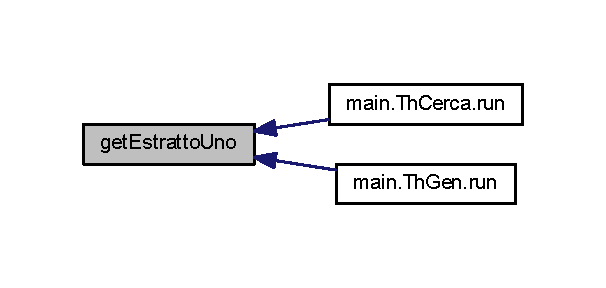
\includegraphics[width=291pt]{classmain_1_1_shared_data_a113b8bd4e0520f7610c30c826d177898_icgraph}
\end{center}
\end{figure}
\mbox{\Hypertarget{classmain_1_1_shared_data_ab9a75de14be42bfeb3654d44f09b20bf}\label{classmain_1_1_shared_data_ab9a75de14be42bfeb3654d44f09b20bf}} 
\index{main\+::\+Shared\+Data@{main\+::\+Shared\+Data}!get\+Fine\+Semaphore@{get\+Fine\+Semaphore}}
\index{get\+Fine\+Semaphore@{get\+Fine\+Semaphore}!main\+::\+Shared\+Data@{main\+::\+Shared\+Data}}
\subsubsection{\texorpdfstring{get\+Fine\+Semaphore()}{getFineSemaphore()}}
{\footnotesize\ttfamily synchronized Semaphore get\+Fine\+Semaphore (\begin{DoxyParamCaption}{ }\end{DoxyParamCaption})}



Definition at line 46 of file Shared\+Data.\+java.

Here is the caller graph for this function\+:
\nopagebreak
\begin{figure}[H]
\begin{center}
\leavevmode
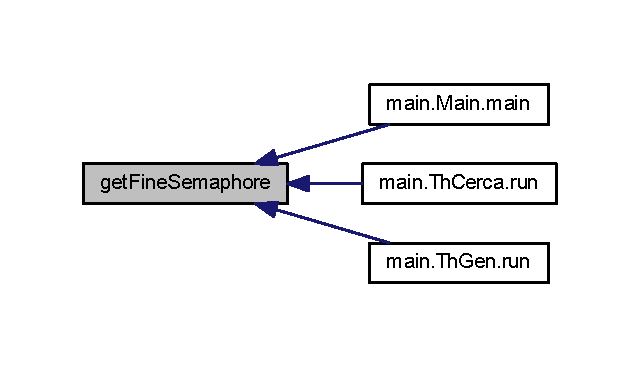
\includegraphics[width=307pt]{classmain_1_1_shared_data_ab9a75de14be42bfeb3654d44f09b20bf_icgraph}
\end{center}
\end{figure}
\mbox{\Hypertarget{classmain_1_1_shared_data_a61e4168cef037c5305a703af0c3e5ce5}\label{classmain_1_1_shared_data_a61e4168cef037c5305a703af0c3e5ce5}} 
\index{main\+::\+Shared\+Data@{main\+::\+Shared\+Data}!get\+Punatato\+Uno@{get\+Punatato\+Uno}}
\index{get\+Punatato\+Uno@{get\+Punatato\+Uno}!main\+::\+Shared\+Data@{main\+::\+Shared\+Data}}
\subsubsection{\texorpdfstring{get\+Punatato\+Uno()}{getPunatatoUno()}}
{\footnotesize\ttfamily synchronized int get\+Punatato\+Uno (\begin{DoxyParamCaption}{ }\end{DoxyParamCaption})}



Definition at line 34 of file Shared\+Data.\+java.

Here is the caller graph for this function\+:
\nopagebreak
\begin{figure}[H]
\begin{center}
\leavevmode
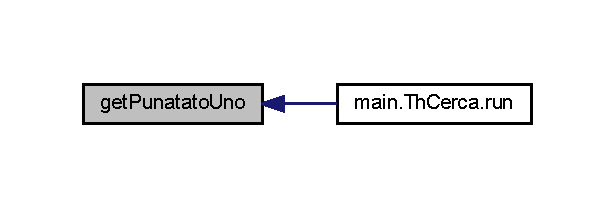
\includegraphics[width=295pt]{classmain_1_1_shared_data_a61e4168cef037c5305a703af0c3e5ce5_icgraph}
\end{center}
\end{figure}
\mbox{\Hypertarget{classmain_1_1_shared_data_afe476c2ad5a76e2d77871f0cfe94b1fd}\label{classmain_1_1_shared_data_afe476c2ad5a76e2d77871f0cfe94b1fd}} 
\index{main\+::\+Shared\+Data@{main\+::\+Shared\+Data}!get\+Puntato\+Due@{get\+Puntato\+Due}}
\index{get\+Puntato\+Due@{get\+Puntato\+Due}!main\+::\+Shared\+Data@{main\+::\+Shared\+Data}}
\subsubsection{\texorpdfstring{get\+Puntato\+Due()}{getPuntatoDue()}}
{\footnotesize\ttfamily synchronized int get\+Puntato\+Due (\begin{DoxyParamCaption}{ }\end{DoxyParamCaption})}



Definition at line 38 of file Shared\+Data.\+java.

Here is the caller graph for this function\+:
\nopagebreak
\begin{figure}[H]
\begin{center}
\leavevmode
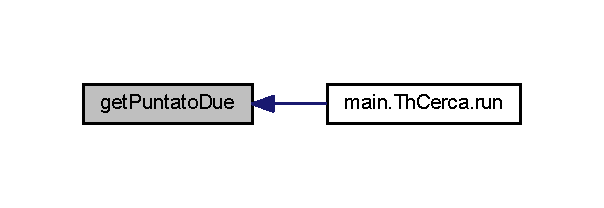
\includegraphics[width=290pt]{classmain_1_1_shared_data_afe476c2ad5a76e2d77871f0cfe94b1fd_icgraph}
\end{center}
\end{figure}
\mbox{\Hypertarget{classmain_1_1_shared_data_aa492c5b4f3fb55eb33f9c79b7b484d41}\label{classmain_1_1_shared_data_aa492c5b4f3fb55eb33f9c79b7b484d41}} 
\index{main\+::\+Shared\+Data@{main\+::\+Shared\+Data}!get\+Ruote@{get\+Ruote}}
\index{get\+Ruote@{get\+Ruote}!main\+::\+Shared\+Data@{main\+::\+Shared\+Data}}
\subsubsection{\texorpdfstring{get\+Ruote()}{getRuote()}}
{\footnotesize\ttfamily synchronized Vector$<$\mbox{\hyperlink{classmain_1_1_ruota}{Ruota}}$>$ get\+Ruote (\begin{DoxyParamCaption}{ }\end{DoxyParamCaption})}



Definition at line 42 of file Shared\+Data.\+java.

Here is the caller graph for this function\+:
\nopagebreak
\begin{figure}[H]
\begin{center}
\leavevmode
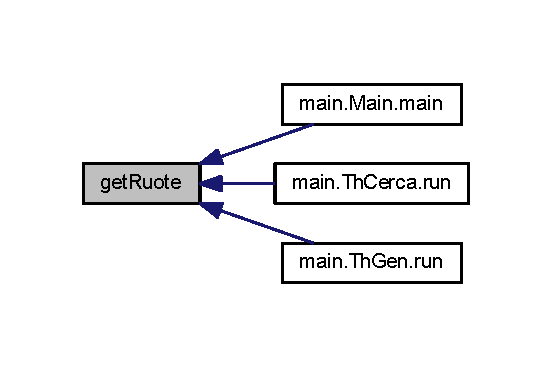
\includegraphics[width=265pt]{classmain_1_1_shared_data_aa492c5b4f3fb55eb33f9c79b7b484d41_icgraph}
\end{center}
\end{figure}


\subsection{Member Data Documentation}
\mbox{\Hypertarget{classmain_1_1_shared_data_a63712f23e96673948c3fd3c48b64d05b}\label{classmain_1_1_shared_data_a63712f23e96673948c3fd3c48b64d05b}} 
\index{main\+::\+Shared\+Data@{main\+::\+Shared\+Data}!estratto\+Uno@{estratto\+Uno}}
\index{estratto\+Uno@{estratto\+Uno}!main\+::\+Shared\+Data@{main\+::\+Shared\+Data}}
\subsubsection{\texorpdfstring{estratto\+Uno}{estrattoUno}}
{\footnotesize\ttfamily final Semaphore estratto\+Uno\hspace{0.3cm}{\ttfamily [private]}}



Definition at line 11 of file Shared\+Data.\+java.

\mbox{\Hypertarget{classmain_1_1_shared_data_af9e82eed5f04a857c2749dae6956ddc1}\label{classmain_1_1_shared_data_af9e82eed5f04a857c2749dae6956ddc1}} 
\index{main\+::\+Shared\+Data@{main\+::\+Shared\+Data}!M\+A\+X\+\_\+\+N\+U\+M\+E\+RO@{M\+A\+X\+\_\+\+N\+U\+M\+E\+RO}}
\index{M\+A\+X\+\_\+\+N\+U\+M\+E\+RO@{M\+A\+X\+\_\+\+N\+U\+M\+E\+RO}!main\+::\+Shared\+Data@{main\+::\+Shared\+Data}}
\subsubsection{\texorpdfstring{M\+A\+X\+\_\+\+N\+U\+M\+E\+RO}{MAX\_NUMERO}}
{\footnotesize\ttfamily final int M\+A\+X\+\_\+\+N\+U\+M\+E\+RO = 99\hspace{0.3cm}{\ttfamily [static]}}



Definition at line 8 of file Shared\+Data.\+java.

\mbox{\Hypertarget{classmain_1_1_shared_data_afd761d5f372b32a47d35514239540df6}\label{classmain_1_1_shared_data_afd761d5f372b32a47d35514239540df6}} 
\index{main\+::\+Shared\+Data@{main\+::\+Shared\+Data}!num\+Ruote@{num\+Ruote}}
\index{num\+Ruote@{num\+Ruote}!main\+::\+Shared\+Data@{main\+::\+Shared\+Data}}
\subsubsection{\texorpdfstring{num\+Ruote}{numRuote}}
{\footnotesize\ttfamily final int num\+Ruote\hspace{0.3cm}{\ttfamily [private]}}



Definition at line 10 of file Shared\+Data.\+java.

\mbox{\Hypertarget{classmain_1_1_shared_data_a3336af22f48845590e6b9cace9d82ce1}\label{classmain_1_1_shared_data_a3336af22f48845590e6b9cace9d82ce1}} 
\index{main\+::\+Shared\+Data@{main\+::\+Shared\+Data}!ruote@{ruote}}
\index{ruote@{ruote}!main\+::\+Shared\+Data@{main\+::\+Shared\+Data}}
\subsubsection{\texorpdfstring{ruote}{ruote}}
{\footnotesize\ttfamily Vector$<$\mbox{\hyperlink{classmain_1_1_ruota}{Ruota}}$>$ ruote\hspace{0.3cm}{\ttfamily [private]}}



Definition at line 9 of file Shared\+Data.\+java.



The documentation for this class was generated from the following file\+:\begin{DoxyCompactItemize}
\item 
C\+:/\+Users/\+Luca Mantica/\+Desktop/\+Scuola/4 anno/\+Tecnologie/\+Java/\+Repositories/\+Lotto/\+Lotto/src/main/\mbox{\hyperlink{_shared_data_8java}{Shared\+Data.\+java}}\end{DoxyCompactItemize}

\hypertarget{classmain_1_1_th_cerca}{}\section{Th\+Cerca Class Reference}
\label{classmain_1_1_th_cerca}\index{Th\+Cerca@{Th\+Cerca}}


Inheritance diagram for Th\+Cerca\+:
\nopagebreak
\begin{figure}[H]
\begin{center}
\leavevmode
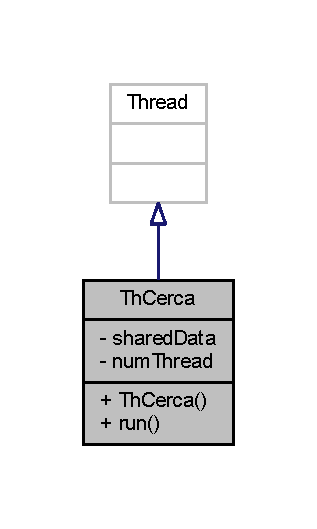
\includegraphics[width=152pt]{classmain_1_1_th_cerca__inherit__graph}
\end{center}
\end{figure}


Collaboration diagram for Th\+Cerca\+:
\nopagebreak
\begin{figure}[H]
\begin{center}
\leavevmode
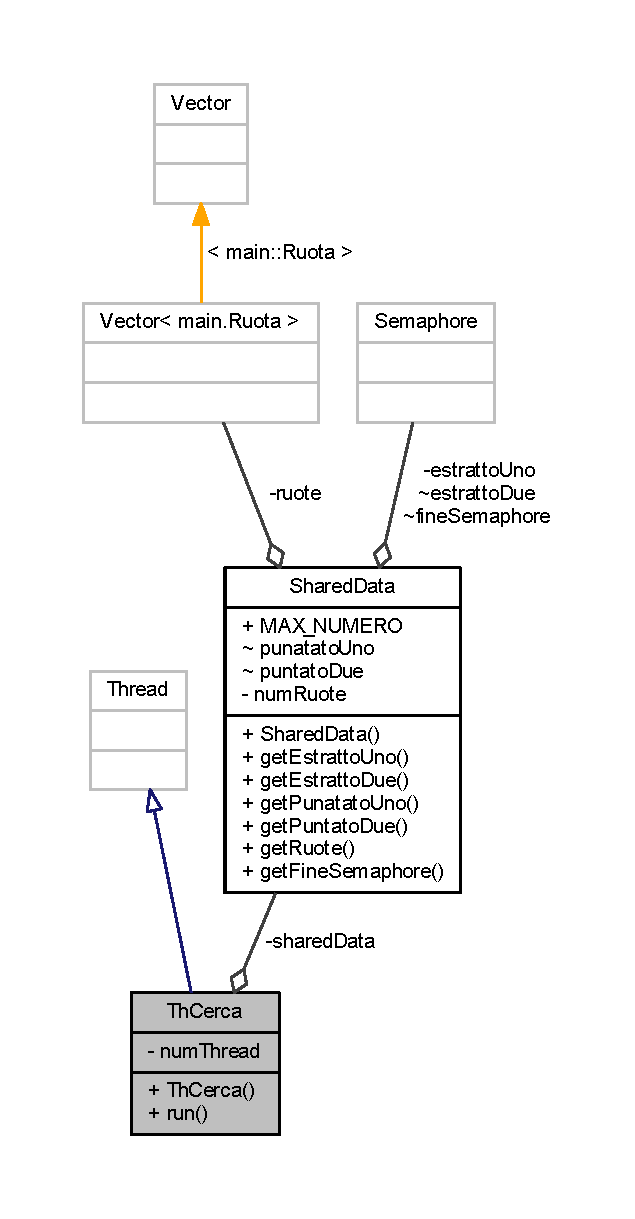
\includegraphics[height=550pt]{classmain_1_1_th_cerca__coll__graph}
\end{center}
\end{figure}
\subsection*{Public Member Functions}
\begin{DoxyCompactItemize}
\item 
\mbox{\hyperlink{classmain_1_1_th_cerca_a0a83c1da759198486023f64ed17596ca}{Th\+Cerca}} (\mbox{\hyperlink{classmain_1_1_shared_data}{Shared\+Data}} \mbox{\hyperlink{classmain_1_1_th_cerca_ac5f1128ef8d0ba91a8214e03732e2662}{shared\+Data}}, int \mbox{\hyperlink{classmain_1_1_th_cerca_a647182b81f9dc0ef69645f81af0b6a73}{num\+Thread}})
\item 
void \mbox{\hyperlink{classmain_1_1_th_cerca_a13a43e6d814de94978c515cb084873b1}{run}} ()
\end{DoxyCompactItemize}
\subsection*{Private Attributes}
\begin{DoxyCompactItemize}
\item 
final \mbox{\hyperlink{classmain_1_1_shared_data}{Shared\+Data}} \mbox{\hyperlink{classmain_1_1_th_cerca_ac5f1128ef8d0ba91a8214e03732e2662}{shared\+Data}}
\item 
final int \mbox{\hyperlink{classmain_1_1_th_cerca_a647182b81f9dc0ef69645f81af0b6a73}{num\+Thread}}
\end{DoxyCompactItemize}


\subsection{Detailed Description}


Definition at line 7 of file Th\+Cerca.\+java.



\subsection{Constructor \& Destructor Documentation}
\mbox{\Hypertarget{classmain_1_1_th_cerca_a0a83c1da759198486023f64ed17596ca}\label{classmain_1_1_th_cerca_a0a83c1da759198486023f64ed17596ca}} 
\index{main\+::\+Th\+Cerca@{main\+::\+Th\+Cerca}!Th\+Cerca@{Th\+Cerca}}
\index{Th\+Cerca@{Th\+Cerca}!main\+::\+Th\+Cerca@{main\+::\+Th\+Cerca}}
\subsubsection{\texorpdfstring{Th\+Cerca()}{ThCerca()}}
{\footnotesize\ttfamily \mbox{\hyperlink{classmain_1_1_th_cerca}{Th\+Cerca}} (\begin{DoxyParamCaption}\item[{\mbox{\hyperlink{classmain_1_1_shared_data}{Shared\+Data}}}]{shared\+Data,  }\item[{int}]{num\+Thread }\end{DoxyParamCaption})}



Definition at line 12 of file Th\+Cerca.\+java.



\subsection{Member Function Documentation}
\mbox{\Hypertarget{classmain_1_1_th_cerca_a13a43e6d814de94978c515cb084873b1}\label{classmain_1_1_th_cerca_a13a43e6d814de94978c515cb084873b1}} 
\index{main\+::\+Th\+Cerca@{main\+::\+Th\+Cerca}!run@{run}}
\index{run@{run}!main\+::\+Th\+Cerca@{main\+::\+Th\+Cerca}}
\subsubsection{\texorpdfstring{run()}{run()}}
{\footnotesize\ttfamily void run (\begin{DoxyParamCaption}{ }\end{DoxyParamCaption})}



Definition at line 18 of file Th\+Cerca.\+java.

Here is the call graph for this function\+:
\nopagebreak
\begin{figure}[H]
\begin{center}
\leavevmode
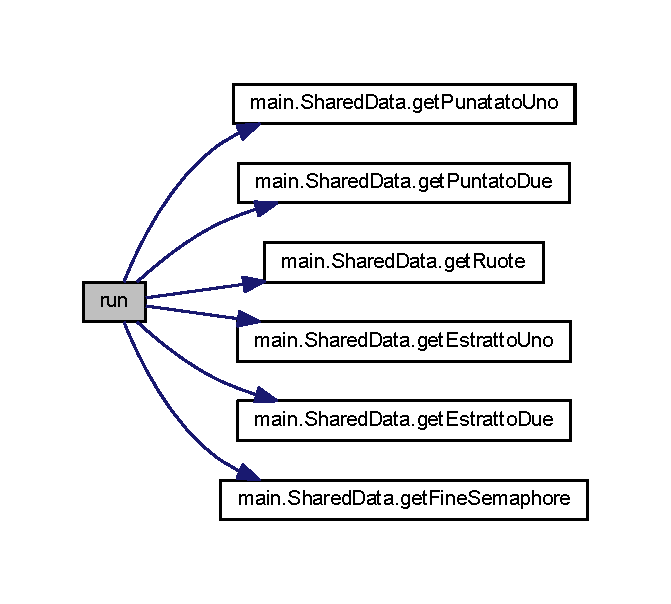
\includegraphics[width=322pt]{classmain_1_1_th_cerca_a13a43e6d814de94978c515cb084873b1_cgraph}
\end{center}
\end{figure}


\subsection{Member Data Documentation}
\mbox{\Hypertarget{classmain_1_1_th_cerca_a647182b81f9dc0ef69645f81af0b6a73}\label{classmain_1_1_th_cerca_a647182b81f9dc0ef69645f81af0b6a73}} 
\index{main\+::\+Th\+Cerca@{main\+::\+Th\+Cerca}!num\+Thread@{num\+Thread}}
\index{num\+Thread@{num\+Thread}!main\+::\+Th\+Cerca@{main\+::\+Th\+Cerca}}
\subsubsection{\texorpdfstring{num\+Thread}{numThread}}
{\footnotesize\ttfamily final int num\+Thread\hspace{0.3cm}{\ttfamily [private]}}



Definition at line 10 of file Th\+Cerca.\+java.

\mbox{\Hypertarget{classmain_1_1_th_cerca_ac5f1128ef8d0ba91a8214e03732e2662}\label{classmain_1_1_th_cerca_ac5f1128ef8d0ba91a8214e03732e2662}} 
\index{main\+::\+Th\+Cerca@{main\+::\+Th\+Cerca}!shared\+Data@{shared\+Data}}
\index{shared\+Data@{shared\+Data}!main\+::\+Th\+Cerca@{main\+::\+Th\+Cerca}}
\subsubsection{\texorpdfstring{shared\+Data}{sharedData}}
{\footnotesize\ttfamily final \mbox{\hyperlink{classmain_1_1_shared_data}{Shared\+Data}} shared\+Data\hspace{0.3cm}{\ttfamily [private]}}



Definition at line 9 of file Th\+Cerca.\+java.



The documentation for this class was generated from the following file\+:\begin{DoxyCompactItemize}
\item 
C\+:/\+Users/\+Luca Mantica/\+Desktop/\+Scuola/4 anno/\+Tecnologie/\+Java/\+Repositories/\+Lotto/\+Lotto/src/main/\mbox{\hyperlink{_th_cerca_8java}{Th\+Cerca.\+java}}\end{DoxyCompactItemize}

\hypertarget{classmain_1_1_th_gen}{}\section{Th\+Gen Class Reference}
\label{classmain_1_1_th_gen}\index{Th\+Gen@{Th\+Gen}}


Inheritance diagram for Th\+Gen\+:
\nopagebreak
\begin{figure}[H]
\begin{center}
\leavevmode
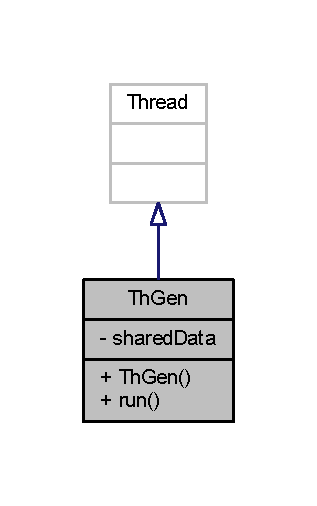
\includegraphics[width=152pt]{classmain_1_1_th_gen__inherit__graph}
\end{center}
\end{figure}


Collaboration diagram for Th\+Gen\+:
\nopagebreak
\begin{figure}[H]
\begin{center}
\leavevmode
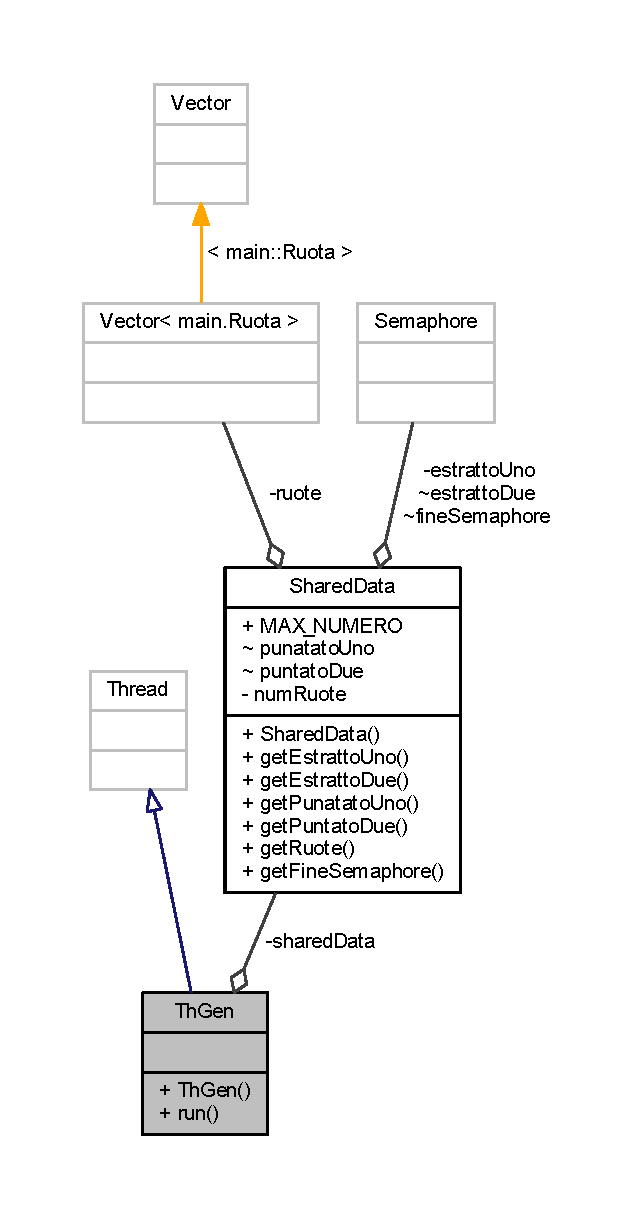
\includegraphics[height=550pt]{classmain_1_1_th_gen__coll__graph}
\end{center}
\end{figure}
\subsection*{Public Member Functions}
\begin{DoxyCompactItemize}
\item 
\mbox{\hyperlink{classmain_1_1_th_gen_ab975ff8819d4ba6b00d6661950d14bb6}{Th\+Gen}} (\mbox{\hyperlink{classmain_1_1_shared_data}{Shared\+Data}} \mbox{\hyperlink{classmain_1_1_th_gen_ac5f1128ef8d0ba91a8214e03732e2662}{shared\+Data}})
\item 
void \mbox{\hyperlink{classmain_1_1_th_gen_a13a43e6d814de94978c515cb084873b1}{run}} ()
\end{DoxyCompactItemize}
\subsection*{Private Attributes}
\begin{DoxyCompactItemize}
\item 
final \mbox{\hyperlink{classmain_1_1_shared_data}{Shared\+Data}} \mbox{\hyperlink{classmain_1_1_th_gen_ac5f1128ef8d0ba91a8214e03732e2662}{shared\+Data}}
\end{DoxyCompactItemize}


\subsection{Detailed Description}


Definition at line 5 of file Th\+Gen.\+java.



\subsection{Constructor \& Destructor Documentation}
\mbox{\Hypertarget{classmain_1_1_th_gen_ab975ff8819d4ba6b00d6661950d14bb6}\label{classmain_1_1_th_gen_ab975ff8819d4ba6b00d6661950d14bb6}} 
\index{main\+::\+Th\+Gen@{main\+::\+Th\+Gen}!Th\+Gen@{Th\+Gen}}
\index{Th\+Gen@{Th\+Gen}!main\+::\+Th\+Gen@{main\+::\+Th\+Gen}}
\subsubsection{\texorpdfstring{Th\+Gen()}{ThGen()}}
{\footnotesize\ttfamily \mbox{\hyperlink{classmain_1_1_th_gen}{Th\+Gen}} (\begin{DoxyParamCaption}\item[{\mbox{\hyperlink{classmain_1_1_shared_data}{Shared\+Data}}}]{shared\+Data }\end{DoxyParamCaption})}



Definition at line 9 of file Th\+Gen.\+java.



\subsection{Member Function Documentation}
\mbox{\Hypertarget{classmain_1_1_th_gen_a13a43e6d814de94978c515cb084873b1}\label{classmain_1_1_th_gen_a13a43e6d814de94978c515cb084873b1}} 
\index{main\+::\+Th\+Gen@{main\+::\+Th\+Gen}!run@{run}}
\index{run@{run}!main\+::\+Th\+Gen@{main\+::\+Th\+Gen}}
\subsubsection{\texorpdfstring{run()}{run()}}
{\footnotesize\ttfamily void run (\begin{DoxyParamCaption}{ }\end{DoxyParamCaption})}



Definition at line 14 of file Th\+Gen.\+java.

Here is the call graph for this function\+:
\nopagebreak
\begin{figure}[H]
\begin{center}
\leavevmode
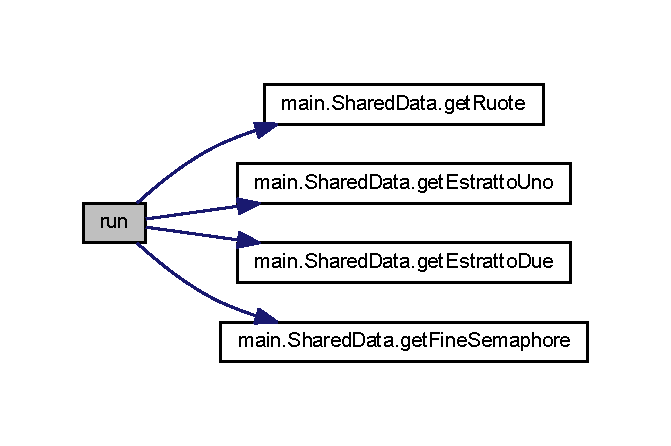
\includegraphics[width=322pt]{classmain_1_1_th_gen_a13a43e6d814de94978c515cb084873b1_cgraph}
\end{center}
\end{figure}


\subsection{Member Data Documentation}
\mbox{\Hypertarget{classmain_1_1_th_gen_ac5f1128ef8d0ba91a8214e03732e2662}\label{classmain_1_1_th_gen_ac5f1128ef8d0ba91a8214e03732e2662}} 
\index{main\+::\+Th\+Gen@{main\+::\+Th\+Gen}!shared\+Data@{shared\+Data}}
\index{shared\+Data@{shared\+Data}!main\+::\+Th\+Gen@{main\+::\+Th\+Gen}}
\subsubsection{\texorpdfstring{shared\+Data}{sharedData}}
{\footnotesize\ttfamily final \mbox{\hyperlink{classmain_1_1_shared_data}{Shared\+Data}} shared\+Data\hspace{0.3cm}{\ttfamily [private]}}



Definition at line 6 of file Th\+Gen.\+java.



The documentation for this class was generated from the following file\+:\begin{DoxyCompactItemize}
\item 
C\+:/\+Users/\+Luca Mantica/\+Desktop/\+Scuola/4 anno/\+Tecnologie/\+Java/\+Repositories/\+Lotto/\+Lotto/src/main/\mbox{\hyperlink{_th_gen_8java}{Th\+Gen.\+java}}\end{DoxyCompactItemize}

\chapter{File Documentation}
\hypertarget{_main_8java}{}\section{C\+:/\+Users/\+Luca Mantica/\+Desktop/\+Scuola/4 anno/\+Tecnologie/\+Java/\+Repositories/\+Lotto/\+Lotto/src/main/\+Main.java File Reference}
\label{_main_8java}\index{C\+:/\+Users/\+Luca Mantica/\+Desktop/\+Scuola/4 anno/\+Tecnologie/\+Java/\+Repositories/\+Lotto/\+Lotto/src/main/\+Main.\+java@{C\+:/\+Users/\+Luca Mantica/\+Desktop/\+Scuola/4 anno/\+Tecnologie/\+Java/\+Repositories/\+Lotto/\+Lotto/src/main/\+Main.\+java}}
\subsection*{Classes}
\begin{DoxyCompactItemize}
\item 
class \mbox{\hyperlink{classmain_1_1_main}{Main}}
\end{DoxyCompactItemize}
\subsection*{Packages}
\begin{DoxyCompactItemize}
\item 
package \mbox{\hyperlink{namespacemain}{main}}
\end{DoxyCompactItemize}

\hypertarget{_ruota_8java}{}\section{C\+:/\+Users/\+Luca Mantica/\+Desktop/\+Scuola/4 anno/\+Tecnologie/\+Java/\+Repositories/\+Lotto/\+Lotto/src/main/\+Ruota.java File Reference}
\label{_ruota_8java}\index{C\+:/\+Users/\+Luca Mantica/\+Desktop/\+Scuola/4 anno/\+Tecnologie/\+Java/\+Repositories/\+Lotto/\+Lotto/src/main/\+Ruota.\+java@{C\+:/\+Users/\+Luca Mantica/\+Desktop/\+Scuola/4 anno/\+Tecnologie/\+Java/\+Repositories/\+Lotto/\+Lotto/src/main/\+Ruota.\+java}}
\subsection*{Classes}
\begin{DoxyCompactItemize}
\item 
class \mbox{\hyperlink{classmain_1_1_ruota}{Ruota}}
\end{DoxyCompactItemize}
\subsection*{Packages}
\begin{DoxyCompactItemize}
\item 
package \mbox{\hyperlink{namespacemain}{main}}
\end{DoxyCompactItemize}

\hypertarget{_shared_data_8java}{}\section{C\+:/\+Users/\+Luca Mantica/\+Desktop/\+Scuola/4 anno/\+Tecnologie/\+Java/\+Repositories/\+Lotto/\+Lotto/src/main/\+Shared\+Data.java File Reference}
\label{_shared_data_8java}\index{C\+:/\+Users/\+Luca Mantica/\+Desktop/\+Scuola/4 anno/\+Tecnologie/\+Java/\+Repositories/\+Lotto/\+Lotto/src/main/\+Shared\+Data.\+java@{C\+:/\+Users/\+Luca Mantica/\+Desktop/\+Scuola/4 anno/\+Tecnologie/\+Java/\+Repositories/\+Lotto/\+Lotto/src/main/\+Shared\+Data.\+java}}
\subsection*{Classes}
\begin{DoxyCompactItemize}
\item 
class \mbox{\hyperlink{classmain_1_1_shared_data}{Shared\+Data}}
\end{DoxyCompactItemize}
\subsection*{Packages}
\begin{DoxyCompactItemize}
\item 
package \mbox{\hyperlink{namespacemain}{main}}
\end{DoxyCompactItemize}

\hypertarget{_th_cerca_8java}{}\section{C\+:/\+Users/\+Luca Mantica/\+Desktop/\+Scuola/4 anno/\+Tecnologie/\+Java/\+Repositories/\+Lotto/\+Lotto/src/main/\+Th\+Cerca.java File Reference}
\label{_th_cerca_8java}\index{C\+:/\+Users/\+Luca Mantica/\+Desktop/\+Scuola/4 anno/\+Tecnologie/\+Java/\+Repositories/\+Lotto/\+Lotto/src/main/\+Th\+Cerca.\+java@{C\+:/\+Users/\+Luca Mantica/\+Desktop/\+Scuola/4 anno/\+Tecnologie/\+Java/\+Repositories/\+Lotto/\+Lotto/src/main/\+Th\+Cerca.\+java}}
\subsection*{Classes}
\begin{DoxyCompactItemize}
\item 
class \mbox{\hyperlink{classmain_1_1_th_cerca}{Th\+Cerca}}
\end{DoxyCompactItemize}
\subsection*{Packages}
\begin{DoxyCompactItemize}
\item 
package \mbox{\hyperlink{namespacemain}{main}}
\end{DoxyCompactItemize}

\hypertarget{_th_gen_8java}{}\section{C\+:/\+Users/\+Luca Mantica/\+Desktop/\+Scuola/4 anno/\+Tecnologie/\+Java/\+Repositories/\+Lotto/\+Lotto/src/main/\+Th\+Gen.java File Reference}
\label{_th_gen_8java}\index{C\+:/\+Users/\+Luca Mantica/\+Desktop/\+Scuola/4 anno/\+Tecnologie/\+Java/\+Repositories/\+Lotto/\+Lotto/src/main/\+Th\+Gen.\+java@{C\+:/\+Users/\+Luca Mantica/\+Desktop/\+Scuola/4 anno/\+Tecnologie/\+Java/\+Repositories/\+Lotto/\+Lotto/src/main/\+Th\+Gen.\+java}}
\subsection*{Classes}
\begin{DoxyCompactItemize}
\item 
class \mbox{\hyperlink{classmain_1_1_th_gen}{Th\+Gen}}
\end{DoxyCompactItemize}
\subsection*{Packages}
\begin{DoxyCompactItemize}
\item 
package \mbox{\hyperlink{namespacemain}{main}}
\end{DoxyCompactItemize}

%--- End generated contents ---

% Index
\backmatter
\newpage
\phantomsection
\clearemptydoublepage
\addcontentsline{toc}{chapter}{Index}
\printindex

\end{document}
